\documentclass[11pt]{article}
%packages

\usepackage{graphicx}
\usepackage{hyperref}

\addtolength{\oddsidemargin}{-.875in}
\addtolength{\evensidemargin}{-.875in}
\addtolength{\textwidth}{1.75in}

\addtolength{\topmargin}{-.875in}
\addtolength{\textheight}{1.75in}
\usepackage{setspace}
\usepackage{float}




\begin{document}


\title{7CCSMGPR GROUP PROJECT FINAL REPORT}
\author{
Lucky Group:\\
  \and
  Robinson, Thomas James\\
  \texttt{1880679}
  \and
  Zhu, Tianning \\
  \texttt{1817456}
  \and
   Sarosi, Marcell \\
  \texttt{1542196}
  \and
  Choi, Daeun \\
  \texttt{1821307}
  \and
  Wu, Zihao \\
  \texttt{1836287}
  \and
  Fu, Yixin \\
  \texttt{1862819}
}

\doublespacing
\date{\today}
\maketitle

\pagebreak


\onehalfspacing
\tableofcontents
\doublespacing

\pagebreak



\section{Introduction}

\subsection{Context}



For the last 12 weeks Lucky Group have been developing a Multi-Host File Synchroniser which is accessible on a mobile application and from a desktop. The want for multi-host file systems has increased dramatically with the development of the web; allowing people to collaborate on complex projects means that there is a greater pool of knowledge contributing, which in turn leads to greater work being produced and in less time. As well as allowing more people to contribute to a project, a multi-host system also allows people to work on their projects from wherever they are as long as they have an internet connection. This further aids the ability of home-based teleworking, which has been found to increase productivity and decrease job attrition by over 50 percent (Bloom, Liang, Roberts,  Ying, 2015). As multi-host systems allow remote access to files and as companies are looking to decrease overhead at every point, this kind of system (which increases flexibility for employers and employees) is significantly increasing the possibility of removing the need for a physical office location. This is just one of the reasons they are becoming so popular. 

Another reason multi-host systems’ popularity is increasing is teamwork. One of the main aspects of working as a team, especially if working remotely, is consistency. Each user must be working from the latest version of the document and be updated with new content as and when it is needed. This is where the synchronisation becomes important. Synchronisation means every user on the system can see where the project is currently at. This also allows management to make more informed decisions to keep the project on track. Synchronisation is the key to allowing multiple users to access the same document at the same time without corrupting the master file when the two versions are uploaded. Systems can do this by scanning documents to see the changes and then merging them. Depending on the rules set when the system is created, additions and deletions will be made to the master document as each user uploads their version. There are a few ways this can be executed, and the choice made will depend on the user’s needs for the system. These methods will be discussed later in the report.

Synchronisation is the solution to the problems when working on multiple hosts, there needs to be a way in which users can be confident that they have data that is consistent with the rest of their team and that when they make changes to the project, their changes will be transferred to the rest of their team without any errors or deletion of any work that is still relevant to the system.

\subsection{Summary of Achievements}

As a group we have achieved the completion of a mobile application and a desktop application that will allow users to upload and download documents to and from their own internal storage. After downloading a file from either application, the user can edit the document in whatever way they please. When they have finished editing, the file can be re-uploaded under the same file name, at this point the system will identify any changes have been made and update the file on the system with the latest version of the document. If there is a conflict of two users trying to upload at different times, the most recent upload will take precedence over the older upload, these files will then be available to see in the database. To be able to complete any tasks on our system the user has to log into the system, where they will then be presented with all the files on the system, this is where the cycle of downloading an uploading may occur. 
Along with the completion of the synchroniser we have also created two reports, of which this is one, and given two presentations documenting the implementation and organisation of the project.

\section{Review}

I will now discuss some of the file sharing systems that are currently on the market. These sites are owned by some of the largest technology companies in the world which shows how valuable this kind of system has become. This is evidenced by all of the systems under review having hundreds of millions of users. Many of these systems have free access up to a certain point of data storage, when this point is reached to gain access to more space on their database you must purchase a membership. In this review I will be looking at the positives and negatives in these systems and suggesting ways in which these could be utilised for our system. The systems I am reviewing are mainly aimed at average consumers instead of corporate customers as this is what our system will be directed towards.

\subsection{Google Drive}

The first system to be reviewed is Google Drive, owned and created by Google, which has over one billion users (reported at a Google conference, reported by (Tech Crunch, 2018)). Google Drive offers online and offline platforms in the forms of a website, applications for desktop users on Windows and macOS, and applications for mobile platforms including Android and iOS smartphones and tablets. This platform allows you to store any file you want up to 5 TB per file, with only the first 15 GB being free you must subscribe to Google One to receive additional space (up to 30 TB). Drive also offers editing capabilities directly within the system by including other Google products on the platform. All information (Google, 2019). 

The most interesting feature of Google Drive, that could be implemented onto our system is the ability to directly edit files on the platform without having to download the file to your local disk space. This feature speeds up the process of making simple adjustments to the file as you do not have to go through the upload and download process. This also means that users save room on their local disk and on their bandwidth as the document may be a large file that would affect other users on the same network. One disadvantage of using Drive is that it does not offer offline applications for Linux systems and Windows phone, although these only account for around 2 percent (Net Market Share, 2019) and 1 percent (Statista, 2018) of the average consumer market share respectively, there will still be a large amount of users that will not be able to effectively handle offline file sharing (Figure 1).

\begin{figure}[t]
\caption{Linux Market Share for the past 12 months}
\centering
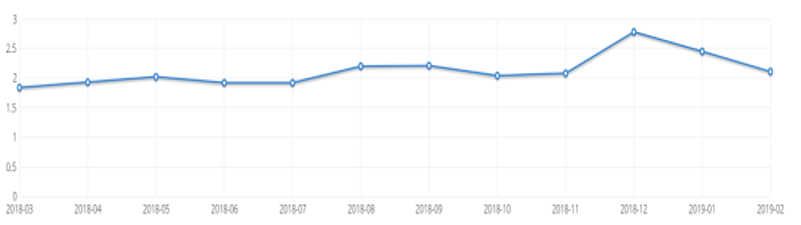
\includegraphics[width=0.8\textwidth]{chart.PNG}
\end{figure}

Another disadvantage to Drive is the way that that you share files with other users, by sending a link to the file or folder that you wish to allow the receiver to edit. This is a disadvantage as the way they have implemented this system (no option to have a password on the links and no expiry dates or download limits) mean that the security of the shared file / folder could be easily compromised.

\subsection{GitHub}

The next system under review will be GitHub. This is now owned and run by Microsoft after acquisition in 2018 (Warren, 2018). It has over 32 million users (GitHub, 2019), making it the largest host of source code in the world  (Gousios, Vasilescu, Serebrenik, \& Zaidman, 2014). GitHub Desktop is the application that allows you to perform GitHub operations without accessing their website. You can also perform all the GitHub features directly in the command line with third party software installed on your system e.g. Git BASH or Git for Windows. There is no official application on either iOS or Android, although there are apps to remove notifications e.g. GitHawk for GitHub. There is no set disk quotas on GitHub, within reason, stating on their website “Keeping repositories small ensures that our servers are fast and downloads are quick for our users.” (GitHub, 2019). GitHub is a more complex file sharing system which is known as a Git repository service. It is often used for sharing projects involving computer code as it offers all the distributed version control and source management functionality of Git.

The main advantages that GitHub has involve its distributed version control. Distributed version control means that you, or anyone who has access to the repository, can update your file from any location allowing for collaboration. Git also allows you to compare changes to a previous version, which means if the program no longer works properly you can compare the changes that were made to the previous version to rectify or revert to the previous version. The other great advantage for GitHub is the branching feature. This feature allows you to make changes to the document in isolation and then merge it with the main branch when you’re sure it works correctly. This means that one user can work on the project at the same time without affecting any other users work, then when they merge to the main line the changes will be implemented independently. These are the features that make GitHub a prime contender for file sharing if the file includes computer code.

One disadvantage of GitHub is the learning curve experienced when first using GitHub. It isn’t as intuitive to use as the other multi-host file synchronisers discussed in this review, with many users claiming it is aimed more at programmers. This means it doesn’t communicate with layman’s so well, meaning many people use the CLI  over the GUI . This is something that this project will try to avoid by having a clean and simple GUI.  

\subsection{Dropbox}

Dropbox will be the next system under review. It is owned and run by Dropbox, Inc, which has over 500 million users (Dropbox, 2016). Dropbox offers offline applications for all three major desktop operating systems and has mobile applications for Android, iOS and Windows Phone. Dropbox can also be set up to have a special folder on the user’s computer of which can be synchronised with Dropbox servers and other computers that have Dropbox installed as well as smartphones with the mobile applications. Dropbox comes with free storage of up to 2 GB, at this point you can upgrade to a paid personal plan which includes 2 TB or a paid plan ‘For Teams’ which have either 3 TB or an unlimited amount of space (Dropbox, 2019). Dropbox only has one native application built into the system, Dropbox Paper, which is essentially for note taking. However, Dropbox does allow for third party apps to connect adding extra functionality.
For Dropbox, the main advantage of this system lies with its file sharing capabilities. Although you must have the file on your local disk as well as on the cloud service, meaning you do not save any disk space on your local file, Dropbox makes use of block level file transfer. This essentially means the only time the whole file is transmitted to the server is the initial upload, with the future edits being uploaded in 4 MB blocks, this means that files should sync faster.

A disadvantage of using Dropbox compared to other systems is the fact that you must use third party applications to edit any documents, although they have Office integration, there are still some office applications that are missing. Another disadvantage is the amount of space and functionality that is granted with the free membership. Although, the pricing, storage and app integration aspects aren’t features that we will be implementing in this project. 

\subsection{OneDrive}

The last system I will be reviewing is OneDrive which is run by Microsoft and again has hundreds of millions of users. OneDrive offers desktop applications for Windows and Mac users, as well as mobile applications for Android and iOS, but not for Linux and Windows Phone users. OneDrive also allows for a folder to be set up in the users file explorer in which you can directly transfer files to the cloud service and this comes as a default on Windows enabled computers. OneDrive comes with 5 GB of free storage, which can be upgraded to 50 GB of storage without any other subscriptions, at this point there are only ‘premium’ accounts. These accounts include other Office 365 applications and offer either 1 TB or 6 TB (for 6 users at 1 TB per person) (Microsoft, 2019). As this is a Microsoft service, Online Office is readily available, as well as OneNote, which is Microsoft’s answer to Dropbox Paper. Any other third-party application integration is harder to come by, although Office does cover most of the essential tasks that you could want to complete without downloading the file. 

A strength that OneDrive has is its file sharing operations, this has a clean and simple mechanism to share and collaborate on projects with other people. With password and expiry date capabilities, you can be sure that the intended recipients are the only person/people that can read the documents. OneDrive also makes use of block level file transfer, although not at the same rate as Dropbox, it still makes for faster upload speeds.

One thing that I have found from personal use of OneDrive is that when the space is full in your OneDrive account there are persistent notifications prompting you to upgrade your account. With the synchronisation a default on Windows systems, this becomes full quickly and this has led me into using another service for cloud storage. Other users have complained about OneDrive struggling to deal with files with hundreds of sub folders and subsequently a large number of files , meaning OneDrive would not be suitable for people with large amounts of data to transfer or for companies to hold their data on.

\section{Requirements \& Design}

This section will outline the requirements we set out to achieve as a group and the reasons we made these decisions. This chapter will also include how the design decisions were affected by the requirements we wanted to fulfil. 
The first requirement decision we made for the system was to decide how to handle what would happen should a conflict of uploads occur. This choice was made at a similar time to the next strategic decision, deciding what should happen when there was a conflict changes depending on whether there was a constant connection with the server or the manual upload method that we settled on. A conflict can be defined as what happens when two users who are working from the same version of a file locally, then proceed to make different changes to the document and then upload. If a conflict occurs we want our system to produce a pop-up that will prompt you to decide between replacing the file in the system or renaming the file with an additional identifier attached to the file name. This will work by using the ‘rsync’ algorithm, which will be further explained in the implementation section.


\begin{figure} [H]
\caption{Initial mockup of system architecture}
\centering
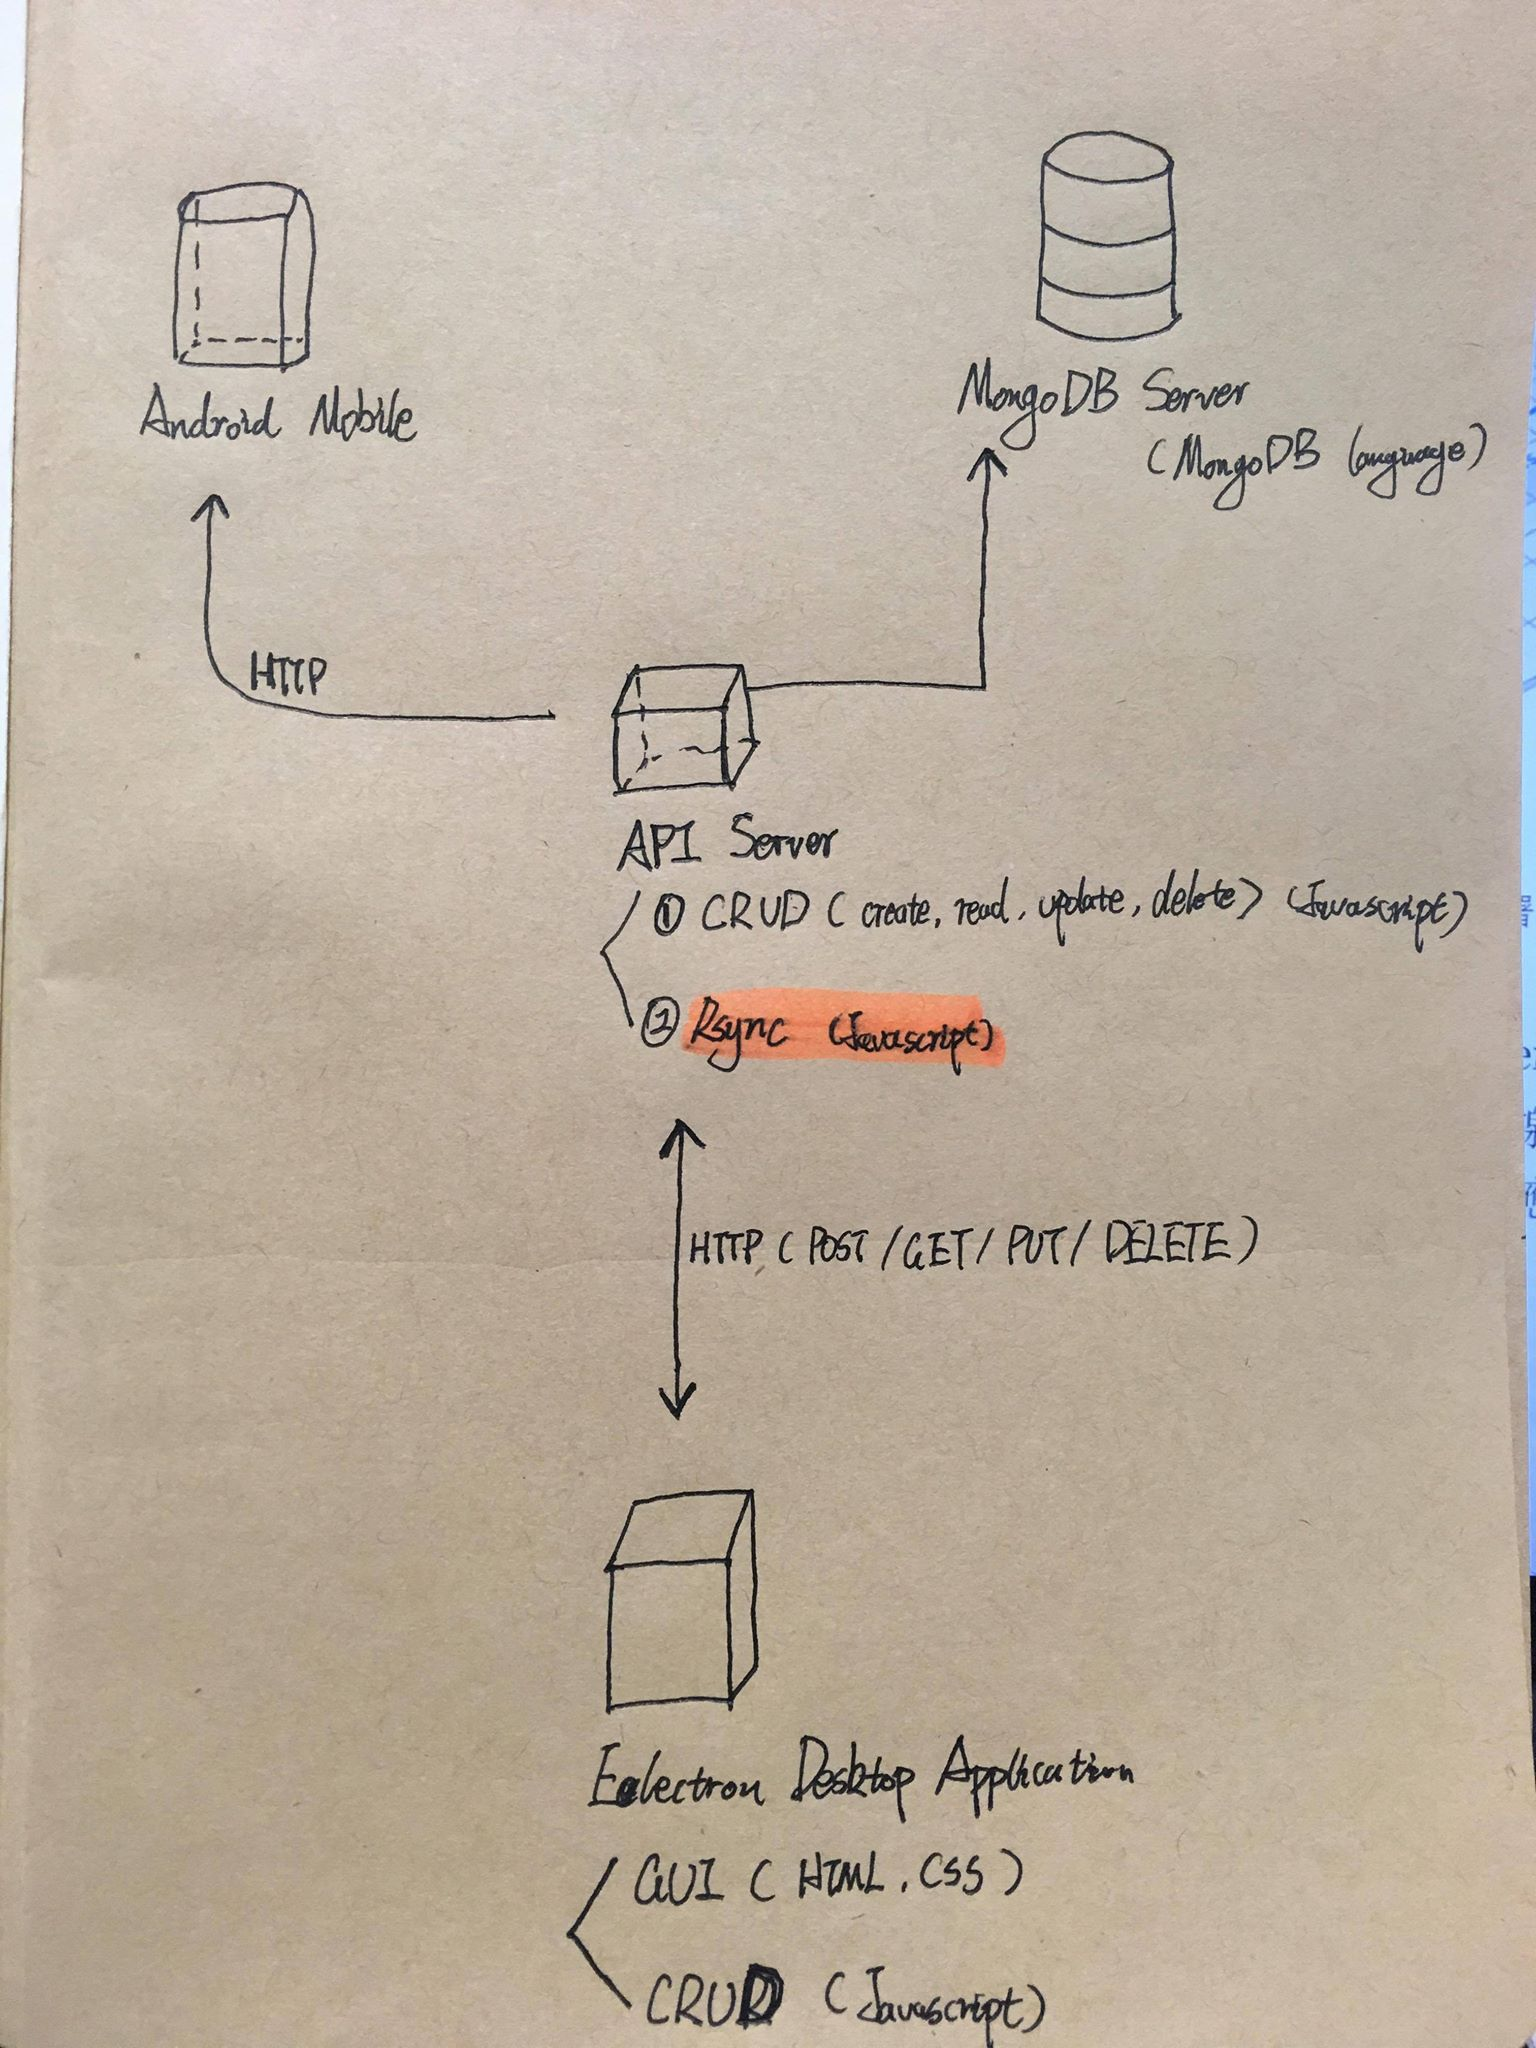
\includegraphics[width=0.6\textwidth]{Group_Project/drawing.jpg}
\end{figure}

Should you choose to replace the file, the document that is currently in the database will be permanently deleted and that version of the file will only be held on the local disk of the user that uploaded that version. We decided to use this method of syncing the files as this allows for more control over the master copy, which means that if someone was unsure if they should be updating the master file, they can save it under a new name. This file can then be reviewed by the team of people working on the project who can, at this point, decide if they want to commit the changes to the master copy. Although this method may lead to an untidier database with multiple copies of the largely similar files, this can quickly be fixed with efficient team work to update the master copy. Another reason we wanted to use this method was that it would be easier to implement a ‘manager’ profile with user access levels. This would allow the system to have an omniscient figure that can ensure that only what is required goes into the latest version of the system and nothing pivotal is deleted. 

This is one of the defining features of our system that deeply affected the rest of the design decisions. If we had decided to use the timed synchronisation method with this strategy, there could be constant stream of uploading new files should there be a conflict with another user working on the file at the same time. This would be an inefficient use of space on the database and would also further increase the strain on the connection as uploading a whole new file every X minutes would take up a lot of bandwidth. There was a discussion within the group about the type of synchronisation that we wanted to implement, with the other option being the master copy being updated with the latest changes. Should a conflict arise using this method the changes would be merged into one document on the system with a mix of the changes implemented on the document. But having decided on using the manual uploading the majority of us agreed that this was the most effective way of handling conflicts as this gives the team more control over what the master copy contains.
The next attribute we discussed as a group was whether we wanted the user to manually upload the file to the system or for there to be a synchronisation update of the file on the system every X minutes (without any action from the user). We came to the decision to keep the responsibility of uploading to the user. The main reason we decided to use this method is because it will provide less opportunity for conflicts to occur, meaning that when the file is overwritten there is less chance of your work being deleted.

If the auto synchronisation method was used with the merging technique mentioned above, files would be deleted as they were being written if two people were writing to the same document at the same time. This could cause confusion for the authors and potential loss of work. This method also doesn’t require a constant connection with the server, allowing for offline work to be completed without exceptions being called. When there is less connection with the server, this is also a benefit for the rest of the network as there is more bandwidth space for other users to perform their tasks. This also means that if a user was to lose connection with the server and close their local version without saving (with them assuming a version had been uploaded to the system), they would lose all their work up to the last upload point or all the work created since opening the file. 

Again, this is one of the main strategic decisions that shaped the outcome and design of the project as this would require less UI for the user to interact with and potentially include a file in the user’s desktop similar to the way that OneDrive and Dropbox do. This would also place a lot of work on the server side of the system, with our experience as coders not being in server-side programming, we decided to keep most of the work being in the user’s application. This decision was made unanimously within our group, with everyone agreeing that this method was the best way for us to proceed.

When you first load our application, you will be presented with a login page. At this point you can either login with a previously registered account, if you don’t already have an account you will have to register with a valid email and matching passwords. We decided we wanted to include user login so each user can have a page which they can see all the files they have uploaded. This would also mean that if someone edits a document already on the system there would be a signature attached to this edit, allowing people to see who changed the document and when. Having user accounts also increases the security of the system as only authorised user will be able to access the database. It also allows us to potentially implement locks on certain documents meaning an author could be able to decide on specific users that can edit a document. 

This decision allowed us to have a more traditional flow of a file sharer and increase security but the design of the system stayed largely the same if there wasn’t a user login at the start of the system. The only difference in design would be depending on if the users have different access levels where one user could have a higher priority when it came to replace the master copy on the database. This level of user could also receive a notification or an email every time someone makes changes to a document that they originally uploaded. The decision to have a login page was unanimously agreed from the start of the project, the use of access levels was also agreed but we decided the implementation of this system was to have a low priority as this is not vital to the core components of the system.

Users of this system will be able to upload any document type to the system; this process occurs on the ‘upload’ page which is accessible from the main menu when the user has passed the login page. There will be looking to implement options to either drag the file directly from the file location open in another program or search their files from a button on the application. When uploading an item, you will be able to add certain footnotes to give other people looking at the item a more information about what is in the folder / document. 

As we have decided to allow any document type to be uploaded to the system, there will not be any function to edit documents directly on the system. This is because there is a vast number of file types that could be uploaded so it would not be possible to implement something that could edit all types of files on this system. The decision not include online editing was agreed within the group to be a low priority and the concentration was to be placed on the core functionality of the system, something that this does not fall under. We are however allowing users to rename files on the system, this works by using a HTTP POST request.
One of the main features of our system, considering we aren’t using within-app editing, is the download function. A user will be able browse all the files they have uploaded and any files that have been made available to see by all the users on the system. When they find the file they want to download, they will be able to inspect the document (read the information provided by uploader), then decide if they want to continue with downloading the item. The user will then be able to decide where they want the file to be saved to. This works by using a HTTP GET request.


\begin{figure} [H]
\caption{The final design for system architecture}
\centering
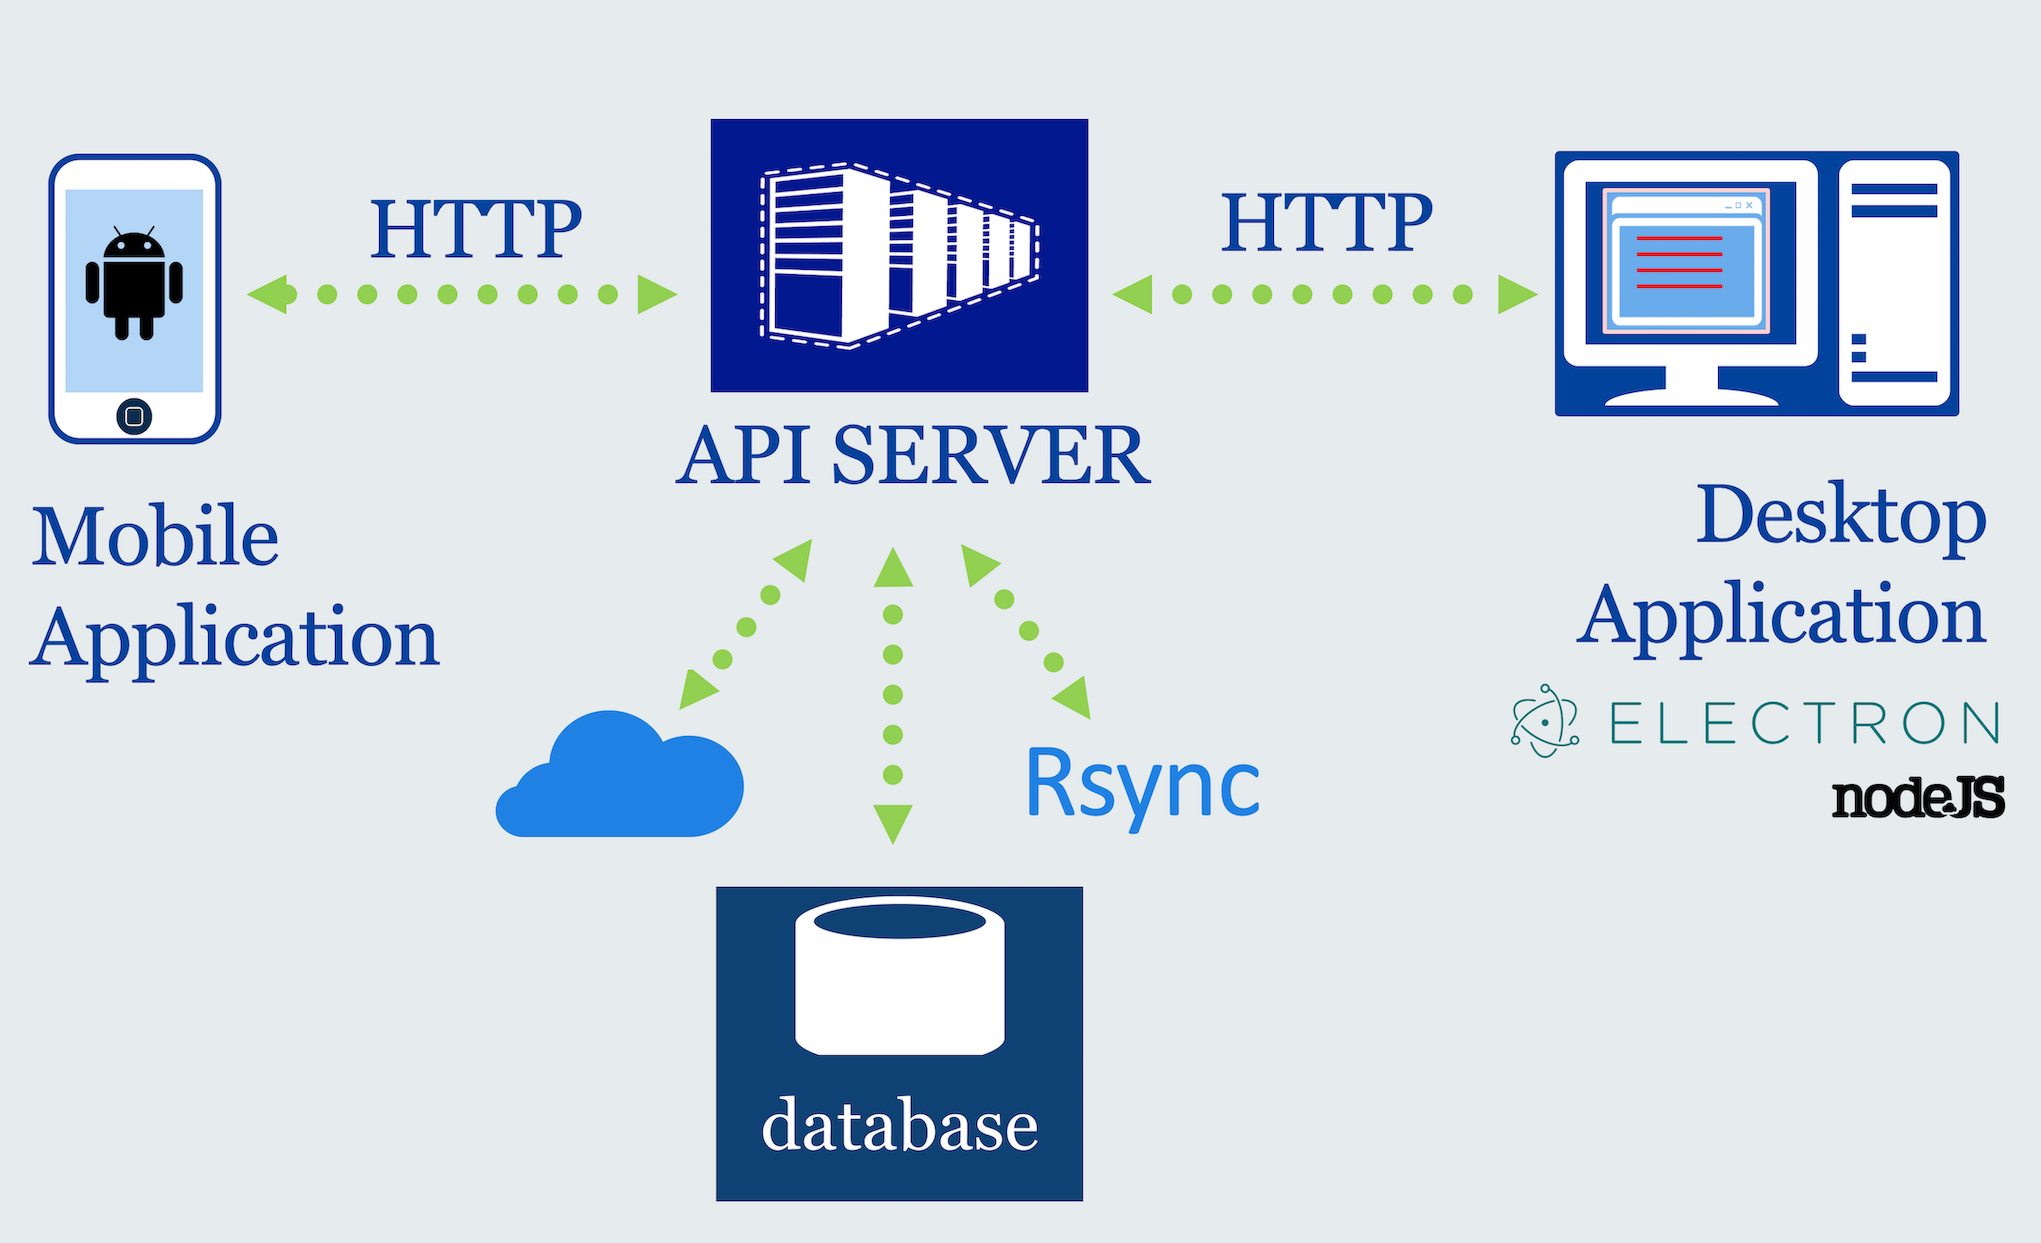
\includegraphics[width=0.9\textwidth]{Group_Project/architecture.png}
\end{figure}

The ability to only see the documents you have uploaded and ones that have been marked public allows a user to have a system that is like GitHub in the sense that when a user is happy with the version they have been working on privately they can reupload to replace the master copy. 

There will also be the option for a user to delete a file from the system if they want to. A user may only delete a file that they have uploaded or edited to prevent a user accidentally deleting another user’s work with a similar title. This may also be implemented with the access levels, meaning that if a user has a ‘manager’ account they may be able to delete all the files in the system as they are trusted to know what is and isn’t important. This works by using a HTTP DELETE request.

We have designed the database to include 3 tables; User, Password, Email and File. The User table will contain a list of usernames, the Password will contain a lift of passwords, the file table will contain information about the files on the system; this includes; size of file and name of file. Other file information is held on the server, here you can see when the file was last updated. At the users end they can affect what is on the database by changing the name of the file and the file size will update according to what is in the file. This information has a bearing on how our synchronisation works, when deciding which file is to take precedence on the system it will look at what the most recent edited file and which file is the largest. This works by using a HTTP GET  request.



\section{Implementation}

\subsection{Analyzing requirements}

The project had 3 key external requirement areas that needed implementation and several pieces of functionality that had to be realised:

\begin{enumerate}
   \item External Requirements
   \begin{itemize}
     \item Hardware: Desktop, Mobile 
     \item Software: This File Synchronise can be compatible with the mobile (Android app) and desktop.
     \item Users: Users need to register their personal details such as name, email to be recorded in the database and login to access to the server for uploading, downloading, deleting files.
   \end{itemize}
   \item Functional Requirements
   \begin{itemize}
     \item Registration: A user needs to register his/her information such as username, password, email in order to access the desktop and mobile application and then the data will be stored in the database to serve as the profile information.
     \item Login: The desktop and mobile application require the user to be registered as the first step to access the system.
     \item Downloading File: A user can download desired files.
     \item Deleting File: A user can delete files that the user wants.
     \item Getting Available File List: A user can get .available file list from server side.
     \item Uploading files to the server
   \end{itemize}
\end{enumerate}


\subsection{Technical Implementation}

\begin{enumerate}
   \item Desktop Application
   \begin{itemize}
     \item \textbf{Electron Framework} : The desktop application of  file synchroniser system is developed by Electron and node.JS.  Electron which is based on web browser and (local) server is an open source library developed by GitHub for building cross-platform desktop applications with HTML, CSS, and JavaScript. Therefore, there are many advantages such as easier implementation for the MVVM pattern and UI customization and graphics, and clear separation between the UI and logic.
   \end{itemize}
   \item Mobile Application
   \begin{itemize}
     \item Fast Android Networking, Android Studio, Download Manger and android-file-chooser: The android app was developed in Android studio using several networking and file management tools. Please see section on android implementation for full details on how the app was constructed and the libraries used.
   \end{itemize}
   \item Server Side Development
   \begin{itemize}
     \item Digital Ocean Cloud Hosting to save files on licensed emote storage
     \item loki.js: an external JavaScript database library was used to help facilite file indexing and storage (http://lokijs.org/.)
     \item rsync-watch-app : Rsync is typically used for synchronizing files and directories between two different systems. This File Synchroniser system uses  rsync-watch-api on server side.
     \item The upload folder will sync to SyncTo folder.
     \item The rsync-watch-app will sync two folders from server side :  a folder from file-upload-api to another one. 
     \item The server application will detect the differences between two folders(temporary folder  and  final folder on the server side), and then, wipe the old version.
     \item The rsync-watch-app will sync two folders from server side :  a folder from file-upload-api to another one. 
     \item We have three server applications : rsync-watch-app, mean-auth-api  and  file-upload-api to provide API to the mobile and desktop to activate the login/register/upload/download/getAllFile/delete.
     \item The server uses REST calls written in node.js to handle all HTTP requests.
     \item Databse items were stored and retrieved using MongoDB, a JavaScript library database solution.
     \item for further details on the server side implementation please refer to code snippets.
   \end{itemize}
   \item Performance issues
   \begin{itemize}
     \item Server Operations:  Server is prone to outages, and on occassions may not respond in time.
    \item Solution : Restarting server, We need to find further proper solution.
    \item Conflicts between File Names
    \item Alert Message : Uploading fail, and Confirm to rename
   \end{itemize}
\end{enumerate}


Please see appendix for more detail on server side code and file structure
  
\subsection{Android Implementation}



\begin{figure} [H]
\caption{RecyclerView with files displayed, a view of the application}
\centering
\includegraphics[width=0.7\textwidth]{files.png}
\end{figure}


The mobile client for the file sharing application was constructed by Marcell Sarosi. Since no member of our group had extensive android development experience, a significant portion of the project runtime had to be devoted to becoming sufficiently proficient in android development to make the application. Development was conducted using Android studio, which is the industry standard tool for creating Android applications. The application code was written in Java.

There were several key user and functional requirements that the mobile client had to address. Users need to be able to register an account for the file sharing service, they have to be able to authenticate themselves to the server. Once logged in users have the option to view the files on the server. Files form the device’s internal storage can be selected and uploaded to the server and equally, files form the server can be downloaded to the device. These requirements clearly indicated that communicating with the sever was the key functionality the app has to realize.

The first step was the creation of the user interface for registration and login as well as for viewing and uploading files. To display the files initially the AndroidTreeNode library ( https://github.com/ bmelnychuk /AndroidTreeView ) was used, which was difficult to work with and was later replaced by a more suitable RecyclerView with a custom built data adapter to show relevant information about the files. A custom file object, FilePojo, was also created to appropriately store data fetched from the server.
To address the communicating with the server through HTTP get and post requests the FAN: Fast Android Networking library (https://github.com/amitshekhariitbhu/Fast-Android-Networking) was added to the project. This allowed for efficient and concise calls to the server and was in most ways the best fit for the project. 


\begin{figure} [H]
\caption{Custom file uploader, replaced by DownloadManager in final product}
\centering
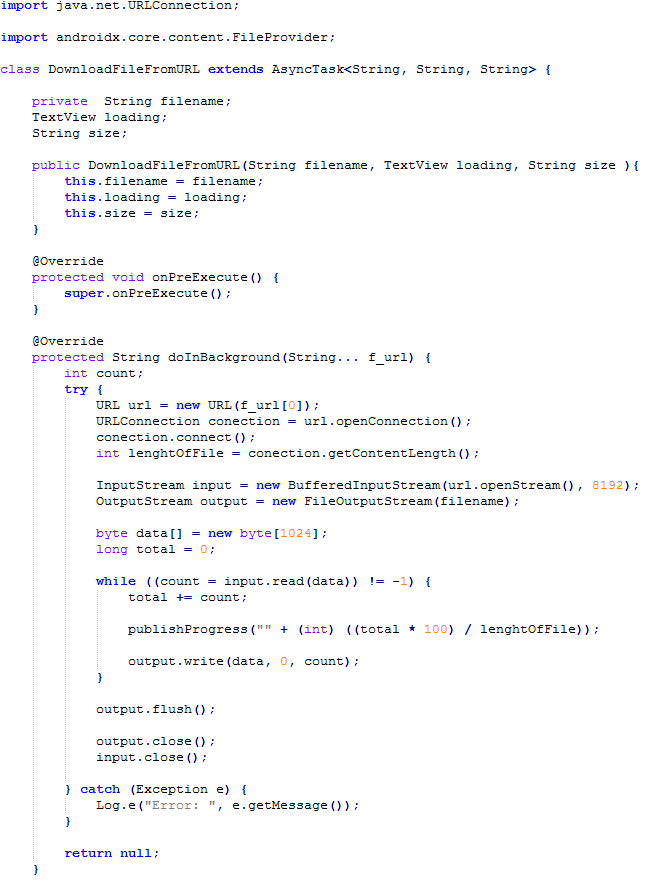
\includegraphics[width=0.8\textwidth]{downloadclass.PNG}
\end{figure}

The application’s main functionality can be categorized into two main groups, user management and file management. In the user management part the key issues are authentication (logging in) and registration. These are both handled through the respective API calls being made to the server containing the data provided by the user. When the user first starts the app he is first taken to the registration page where he can make a new account, the user also has the option to log in with an existing account. After authentication the user profile is saved on the device under shared preferences, and the user will not have to enter his login details again, unless he purposefully logs out of his account. Meaning the user must only type his username and password the first time, and all consequent times he opens up the app, authentication is handled automatically.


The other type of functionality concerns the files located on the server. To display the files the server sends the client a JSON file. This contains the list of files currently stored on the remote storage and information concerning the name, size, metadata and other aspects of the files. This JSON response is then parsed by the mobile client into custom Java objects of type FilePojo, which are then displayed in the UI RecyclerView. 

\begin{figure} [H]
\caption{FAN request to delete a file}
\centering
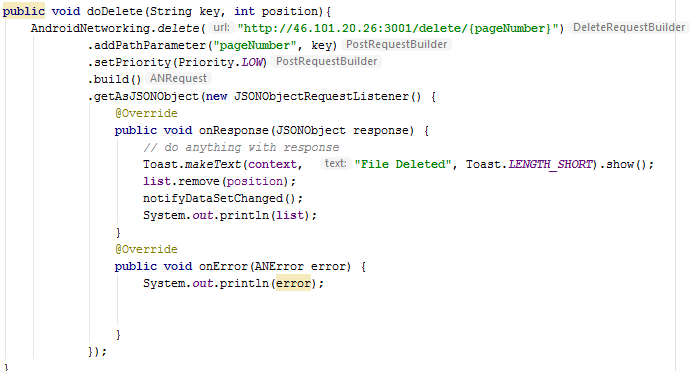
\includegraphics[width=0.8\textwidth]{delete.PNG}
\end{figure}

To download the file the user simply taps on the desired item on the list, a dialogue box is displayed to confirm the download. If the user chooses to download the file a request is sent to the server to fetch file content. One of the main challenges encountered during the Android implementation was constructing a download function which worked efficiently and according to specification. Several approaches were taken to file downloading before the problem was solved. First the default FAN: Fast Android Networking framework was used, but it became apparent that FAN was not the best way to interact with the particular type of file transfer implemented by the server side of the system. After several tries of trying to make the FAN approach work it became clear that a new download method was required. Next a custom file downloader class was constructed using HTTP3 and later URLConnection libraries. While this approach was successful in getting the file data from the server API it was inefficient in its download process and did not give good feedback and options to the user. Finally a suitable file downloading functionality was achieved by integrating Android Download Manager into the application to provide efficient data usage and a familiar user experience. After the file is downloaded the user can open it and edit it in their application of their choosing. For all other HTTP API calls FAN remained our choice of networking framework.


The next part of the application was to implement file uploading. In order to do that the user must have a way of selecting a file from the internal storage of the device to upload. To facilitate file selection the android-file-chooser library (https://github.com/hedzr/android-file-chooser) was used. This is an effective and lightweight solution that enables users to browse their device’s internal memory to select their desired file. The file chooser then passes the file path to the application. If all required upload criteria are met, the file is then sent to the server API in a FAN HTTP Post request encoded as a multipart entity. 
Later in the project the option to delete files was added through a FAN Delete request triggered by holding down on an item and selecting the delete option.


Testing the app was done using Junit4 and espresso, which is standard practice for android testing. The testing verified the presence of the correct components of the application. Additionally communication with the server API was tested using Postman, to verify that the right http requests are being constructed. Testing revealed no faults in the final application code.

All external libraries added in the project and listed below are used under the apache 2.0 license. 

FAN: Fast Android Networking : https://github.com/amitshekhariitbhu/Fast-Android-Networking

	OkHTTP3: https://github.com/square/okhttp
	
android-file-chooser: (https://github.com/hedzr/android-file-chooser)

Please see Appendix for images of Android User Interface.


\section{Team Work}

In this chapter we will be discussing how we worked as a team and what processes and software we used to achieve our final product. Overall, the team worked well together with no major conflicts of personality or opinion in the way to handle the project, this can be attributed to a few reasons. One of the main reasons was that everyone wanted to achieve the same goal, we quickly came to realise this project is very large and complicated which meant that no one person could complete the task successfully without the help from other members. This led us to agree to meet every week, enabling us to discuss what tasks needed completing in the next week as well as discussing the overall aims for the project. It was in one of these meetings towards the end of project one member expressed their concern of using the ‘rsync’ algorithm with the web application. After hearing his reasoning, we decided to change from a website to a desktop application, this was a big change, especially for the front end of the system, and had we not worked efficiently as a team we would not have completed the project in the capacity we did. Although the functionality of the system is not as great as we would have originally liked, the synchronisation works as planned which we felt as a group was the most core feature of the system.

Another reason I think the team worked well was that if someone didn’t understand any part of the project, from GitHub to the logic of our system, someone was readily available to help the person understand what they were struggling with. This could be over Facebook Messenger or in a face to face meeting, which are two of the tools we used to facilitate group work. There were a few occasions near the start of the project in which Yixin took time out of her day to meet with people to help them to get to grips with using GitHub and multiple occasions where Zack met with members to help them understand the detailed logic of the system and help them adapt their code to suit the logic.

The main tool we used for version control was a GitHub repository, as explained earlier GitHub has the best features to deal with computer code due to its ability for identifying changes in multiple user’s code and merge these into the master branch without much input from a ‘leader’ profile (Figure 7). Although there was a learning curve when starting up with GitHub, which was eased by working as a team, the whole group and the project has benefited from the features that GitHub offers over the other file sharing systems.

\begin{figure} [H]
\caption{View of team GitHub Repository}
\centering
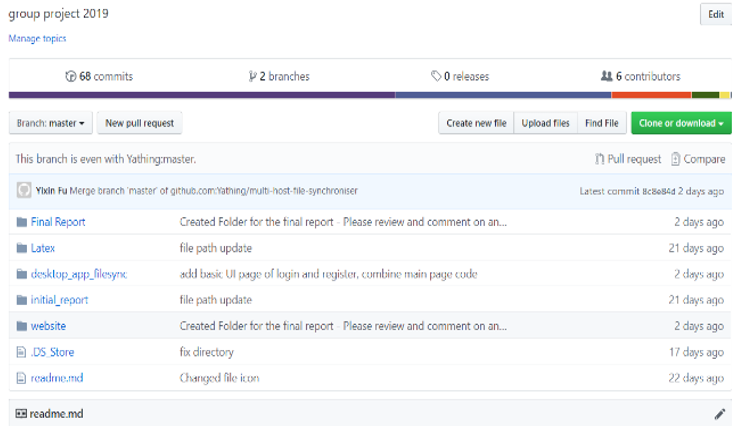
\includegraphics[width=0.8\textwidth]{figure1-1.PNG}
\end{figure}

When it came to write the final report for the project there was a shared Google Drive folder set up for people to collaborate on the word document, this was set up due to the online editing capabilities and being able to see the changes to the document in real time (Figure 8). As the original document is written in Microsoft Word, this allowed the team member converting the document into Latex to do so whenever the file was updated, another example of the team working well together. As well as having these files on Google Drive they were also on our GitHub repository.

\begin{figure} [H]
\caption{View of team Google Drive folders}
\centering
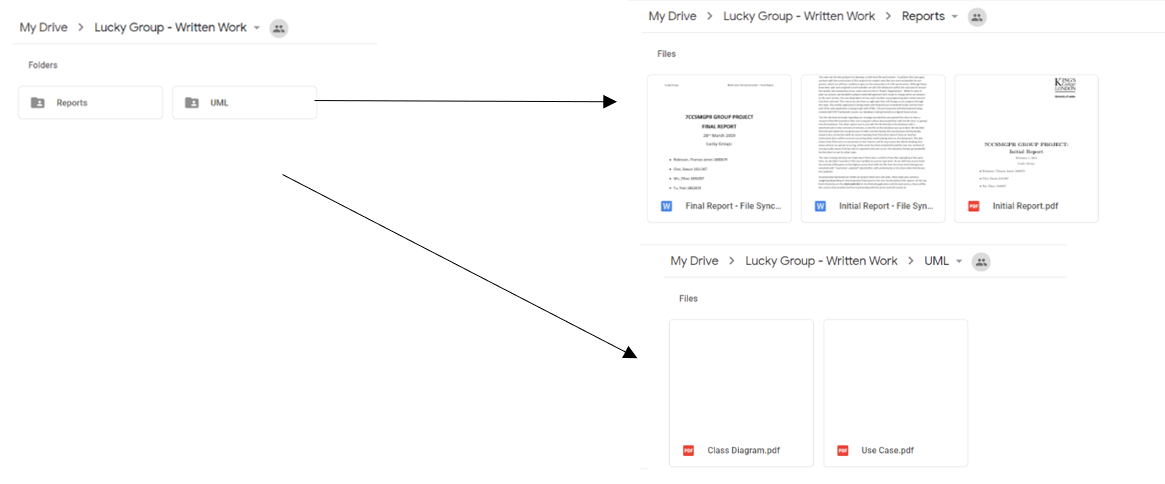
\includegraphics[width=1.0\textwidth]{figure2.PNG}
\end{figure}

Another tool used was Facebook Messenger, this was used for asking questions, updating team members of progress, requesting help, etc. A useful tool in Facebook messenger is the polling feature, this was used on multiple occasions, in the example it is being used to decide on a day for a meeting (Figure 9). 

\begin{figure} [H]
\caption{An example of voting in the group chat}
\centering
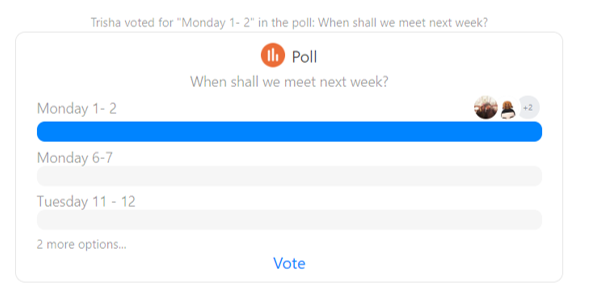
\includegraphics[width=0.7\textwidth]{figure3.PNG}
\end{figure}

\section{Evaluation}

In this section we will discuss the strengths and weaknesses of our system; what we achieved vs the requirements and plan we had at the start of the project, the changes we made to the plan to fit the requirements and any potential future work that could be done to improve the system. I will start by outlining the strengths of our system. 

The main achievement was creating a file system that allows the user to access their files from anywhere with desktop and mobile applications. This was the first goal we set out to accomplish as it the basis for any file sharing system. Although we changed from a website to a desktop application towards the end of the project, we still realised this goal with team play and hard work. Our system works in the way that we set out in the requirements, with the user being able to download a file from the system, edit the document then re-upload it to the server and see the changes implemented in the document available online. The user can also see the size of the file and the date/time the document was uploaded to the server.

Another strength is our login feature, this process means only authorised users can access the file system, increasing security. When the user logs in there will be a check in our database tables to confirm whether there is a match with a username / email with a password. If there is no match the user will be told to create a login and will be directed to the registration page to complete this task. This is the same process as we set out in the requirements for this project.

Server reliability is another part of the project that we completed successfully, this is an important feature for every file hosting system as when the server is unavailable all the documents are unavailable - this is also true with all web-based services and is a key consideration to make before placing your application on the web. We have implemented our server on Digital Ocean.

Our service can also handle all file formats, which is another big positive in our system, this enables the users for any project that they wish, also implementing the notifications to appear with all other notifications on android is something worth mentioning here also. Also, our system will show the user the size of the file and the date the file was uploaded to the system.

Something that worked well was the overall cooperation and understanding of every member of our team, without this there would be no system to review. There were a few testing times in developing this system, as there is to be expected, but the team worked well together to achieve a working system. As a team we all feel like we have learnt valuable lessons about working as a group, especially using GitHub as a tool for collaboration.

One thing that didn’t work well was the splitting of sub-tasks. We initially split into groups for development but the team working on the web application (as it was then) was still large and with no designated leader in the group, people were apprehensive to ask others to complete tasks or create a work flow model. This meant that work was uncoordinated and certain tasks slipped through the cracks, leading to certain members doing a lot of the development work which is of course a slower way of working. This was essentially why the change from web application to desktop application came late in the development process, as the one person working on the API ran into critical trouble concerning the ‘rsync’ algorithm that meant a change in approach was necessary. In future projects it may be beneficial to elect a ‘manager’ or, alternatively, get all the members of a sub team to come together near the start of the project to discuss in detail and devise a timetable outline the tasks need to be completed. 

The biggest change of the plan came when we decided to change from a website to a desktop application, although this changed what the user interacted with, we still had the same logical approach to the problem. We decided to move away from a website and create a desktop as when we were testing on the local host, using the rsync, everything was working correctly, but when we tried to implement on an active server, the synchronisation was taking place between two folders on the server rather than synchronising from the server to the client, this meant that there was no way of updating the server document with from the client side. Another problem we had was providing the php-sync package for the client side, we could not find a way to install this package on every web client.  These problems led us to changing from a website to a desktop application.

One thing we didn’t achieve that we set out at the start of the project was the implementation of authorisation levels. We had placed this at a low priority for the project as it is not part of the core functionality and unfortunately, we have not had the time to implement. Although the system is structured in a way such that, given a bit better planning, we may have had the time to include this functionality. Another thing on the plan that we haven’t implemented is restricting access to other users’ files on the server, as it currently stands all the files on the system are viewable and downloadable for every user. This means, although there a way to see which files you uploaded by themselves, these files will be viewable for everyone on the system. This kind of system would still be acceptable as an internal file system for one company but would severely lack the security features to implement on the internet.

These problems could easily be remedied at a later date, since the architecture of the app was made quite modular and expandable. This is certainly a project that given more time could be worked on further with great ease even by other development teams.

Another thing on the plan that we didn’t implement was the account management part of the system. As we didn’t include the authorisation method there didn’t seem to be any use in having an account management page as there would be nothing on the screen apart from the email they have signed up to the system with. There is also no notifications sent to the user, which was outlined with a low priority in the initial plan.

One weakness of our system is the lack of merging that is allowed. Although we have implemented the way we planned to, the method we have chosen to use doesn’t merge conflicting documents. If two people upload the same document from the same download version one person’s work will be lost from the master file. This is an acceptable method as a user is able to rename their files and this system does have its benefits, which were outlined in the requirements section of this report. There are other benefits associated with having a merger of conflicting documents, which is that it is especially useful for projects that require people to work on different parts of the same project at the same time e.g. projects with computer code. The benefits of this kind of system are similar to the benefits of the GitHub method; distributed version control and branching. 

Another weakness of our system is that no files are editable directly in the application, this means that a user must have space on their disk for the whole file to edit the document in anyway. This means that even if the user only want to add one line to a word document they will have to go through the whole process of downloading and uploading the document. Even when the user has done this there may be a chance that someone is working on another copy of the same version and may overwrite the change implemented by them. This is also a weakness as downloading the whole document may take up space on the on the bandwidth, slowing down other processes on the same network.

Considering the weaknesses and changes to the plan mentioned in this chapter there are is some potential future work that, given time, we could implement into our system. The first potential implementation could be notifying the user if the source file (that they downloaded and started working from) has changed since their download. This would allow the user to make a more informed decision about whether to replace the master or rename the file that they are uploading. This could be extended further by highlighting what changes have been made, either by a word count or highlighting the changes as is done in GitHub. 

The next improvement that could be implemented is the merging of the documents. If the system can identify the changes in the file and bring them to the attention of the uploading user, it could be useful if the user had the option to add their work on-top of the work completed by a collaborator. If it can identify the changes it could be beneficial to include a system that can handle each conflict on a case by case basis, an example of this could be in a word document where paragraphs are analysed one by one, or in computer code function by function. Using this method would give a user more control over the merging of the documents. As well as having an option displayed to the user there could be a managing profile that could authorise all the changes made before committing them to the file on the public database.

One change that could be made to improve the system could be automatically syncing the file with the database. If the merging from the paragraph above had been implemented this process would be a more viable option as the file could be successfully updated with the new work from multiple locations at the same time. On our system currently, this would lead to one of the users’ work being deleted but having both implemented would make the system easier to use for editing less complex files like word documents as it would not require any input from the user. Again since the base system was built for expansion, these functionalities could be implemented later.

A final improvement that would increase the usability of our system would be including a private section on the database for each user to hold their own files without them being visible to other users. This would allow for a kind of ‘branching’ from the master file, with the user being able to make changes to a private version then uploading changes to the master when they are happy with what they have done. This private section would also increase the security of the system, making it more viable to implement outside of just an internal system. This private section also gives the system a more traditional flow of commercial system, with people being able to use the system to store backups of their devices or as a way to store files on the system that they wish to use elsewhere but without anyone else being able to see them.

\section{Peer Assessment}
Here is the breakdown of points allocation, agreed by each member of the group:

\begin{figure} [H]
\caption{The agreed upon score}
\centering
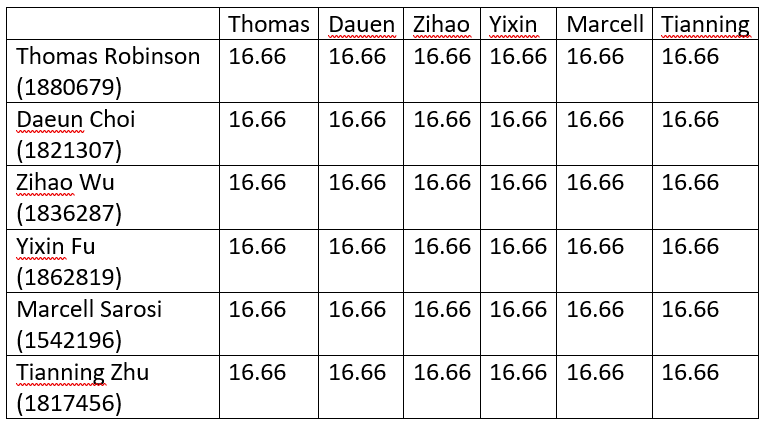
\includegraphics[width=0.7\textwidth]{peer.PNG}
\end{figure}

As it is visible the team has elected to distribute all marks equally amongst the six members.



\begin{thebibliography}{9}
\bibitem{1} 
Bloom, N., Liang, J., Roberts, J., \& Ying, Z. J. (2015). DOES WORKING FROM HOME WORK? EVIDENCE FROM A CHINESE EXPERIMENT*. Retrieved from https://nbloom.people.stanford.edu/sites/g/files/sbiybj4746/f/wfh.pdf
\bibitem{2} 
Dropbox. (2016). Celebrating half a billion users. Retrieved from Dropbox blog: https://blog.dropbox.com/topics/company/500-million
\bibitem{3} 
Bloom, N., Liang, J., Roberts, J., \& Ying, Z. J. (2015). DOES WORKING FROM HOME WORK? EVIDENCE FROM A CHINESE EXPERIMENT*. Retrieved from https://nbloom.people.stanford.edu/sites/g/files/sbiybj4746/f/wfh.pdf
\bibitem{4} 
Dropbox. (2016). Celebrating half a billion users. Retrieved from Dropbox blog: https://blog.dropbox.com/topics/company/500-million
\bibitem{5} 
Dropbox. (2019). The right Dropbox for you. Retrieved from Dropbox: https://www.dropbox.com/plans?oqa=acc\_plan\_upgrade
\bibitem{6} 
GitHub. (2019, April). User Search. Retrieved from GitHub: https://github.com/search?q=type:user\&type=Users
\bibitem{7} 
GitHub. (2019). What is my disk quota? Retrieved from GitHub.Help: https://help.github.com/en/articles/what-is-my-disk-quota
\bibitem{8} 
Google. (2019). Drive Features. Retrieved from https://www.google.com/drive/using-drive/
\bibitem{9} 
Gousios, G., Vasilescu, B., Serebrenik, A., \& Zaidman, A. (2014). Lean GHTorrent: GitHub Data on Demand. MSR 2014 Proceedings of the 11th Working Conference on Mining Software Repositories, 384 -387.
\bibitem{10} 
Microsoft. (2019). One Drive Plans. Retrieved from One Drive: https://onedrive.live.com/about/en-gb/plans/
Net Market Share. (2019). Operating System Market Share. Retrieved from https://netmarketshare.com
\bibitem{11} 
One Drive Community. (2018). onedrive web always stalls/hangs after uploading few files - hangs on "uploading *** items" for ever (win 10 chrome and Edge and IE). Retrieved from One Drive User Voice:
https://onedrive.uservoice.com/forums/913528-onedrive-on-the-web/suggestions/33208225-onedrive-web-always-stalls-hangs-after-uploading-f
\bibitem{12} 
Price, D. (2018). The True Market Shares of Windows vs. Linux Compared. Retrieved from Make Use Of: https://www.makeuseof.com/tag/linux-market-share/
\bibitem{13} 
Smith, C. (2019, March). 20 Amazing GitHub Statistics and Facts 2019 | By the Numbers. Retrieved from DMR:
https://expandedramblings.com/index.php/github-statistics/
\bibitem{14} 
Statista. (2018). Market share of Windows Phone in the United Kingdom (UK) from December 2011 to September 2018. Retrieved from https://www.statista.com/statistics/271255/windows-phone-market-share-in-the-united-kingdom-uk/
\bibitem{15} 
Tech Crunch. (2018). Google Drive will hit a billion users this week. Retrieved from https://techcrunch.com/2018/07/25/google-drive-will-hit-a-billion-users-this-week/guccounter=1\&guce\_referrer\_us=aHR0cHM6Ly93d3cudGhldmVyZ2UuY29tLw 
 \&guce\_referrer\_cs=7TGZhIYb4figcc6zWPN7Bw
\bibitem{16} 
Tutorials Point. (2019). HTTP Requests. Retrieved from Tutorials Point: https://www.tutorialspoint.com/http/http\_requests.htm
Warren, T. (2018). Microsoft completes GitHub acquisition. Retrieved from The Verge: https://www.msn.com/en-us/news/technology/microsoft-completes-github-acquisition/ar-BBOVVOT

\end{thebibliography}

\textbf{Appendix}

\appendix

\section{Libraries}

\begin{itemize}
  \item Lokijs : http://lokijs.org/
  \item Node.JS : https://nodejs.org/en/
  \item MongoDB : https://www.mongodb.com/
  \item Electron : https://electronjs.org/
  \item Fast Android Networking : https://github.com/amitshekhariitbhu/Fast-Android-Networking
  \item OkHTTP3: https://github.com/square/okhttp
  \item android-file-chooser: 
  
  (https://github.com/hedzandroid-file-chooseb.com/hedzr/android-file-chooser)
  \item RSync : https://rsync.samba.org/
\end{itemize}

\section{Server Code}

\setcounter{figure}{0}    

\begin{figure} [H]
\caption{Database Schema for a single file}
\centering
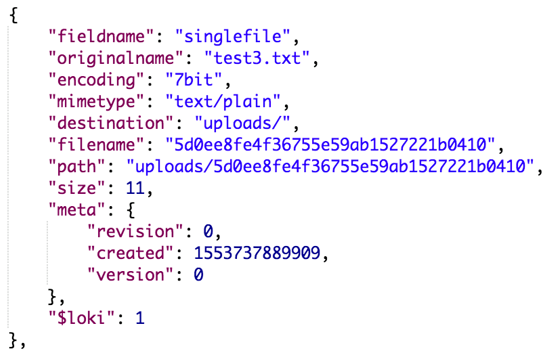
\includegraphics[width=0.7\textwidth]{AFileSchema.PNG}
\end{figure}

\begin{figure} [H]
\caption{Delete API}
\centering
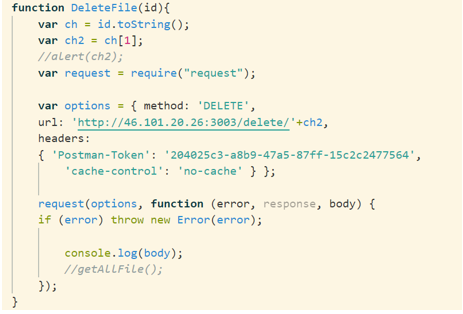
\includegraphics[width=0.7\textwidth]{ADelete.PNG}
\end{figure}

\begin{figure} [H]
\caption{Download API}
\centering
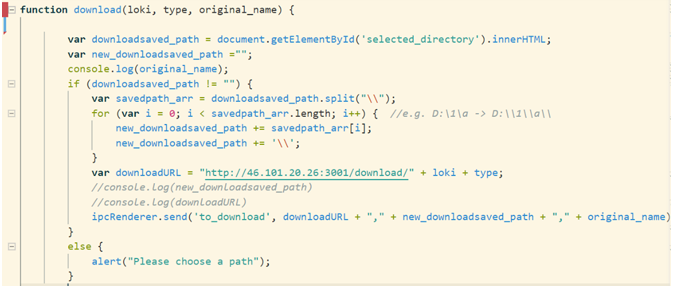
\includegraphics[width=0.7\textwidth]{ADownload.PNG}
\end{figure}

\begin{figure} [H]
\caption{Upload API}
\centering
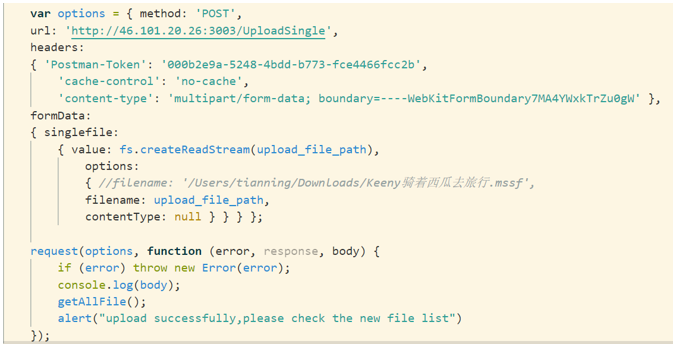
\includegraphics[width=0.7\textwidth]{AUpload.PNG}
\end{figure}

\begin{figure} [H]
\caption{Getfiles API}
\centering
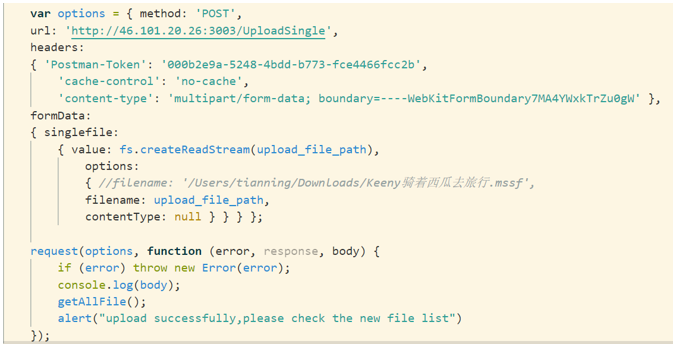
\includegraphics[width=0.7\textwidth]{AUpload.PNG}
\end{figure}

\section{Android UI}

\begin{figure} [H]
\caption{Android UI to log in to application and user account}
\centering
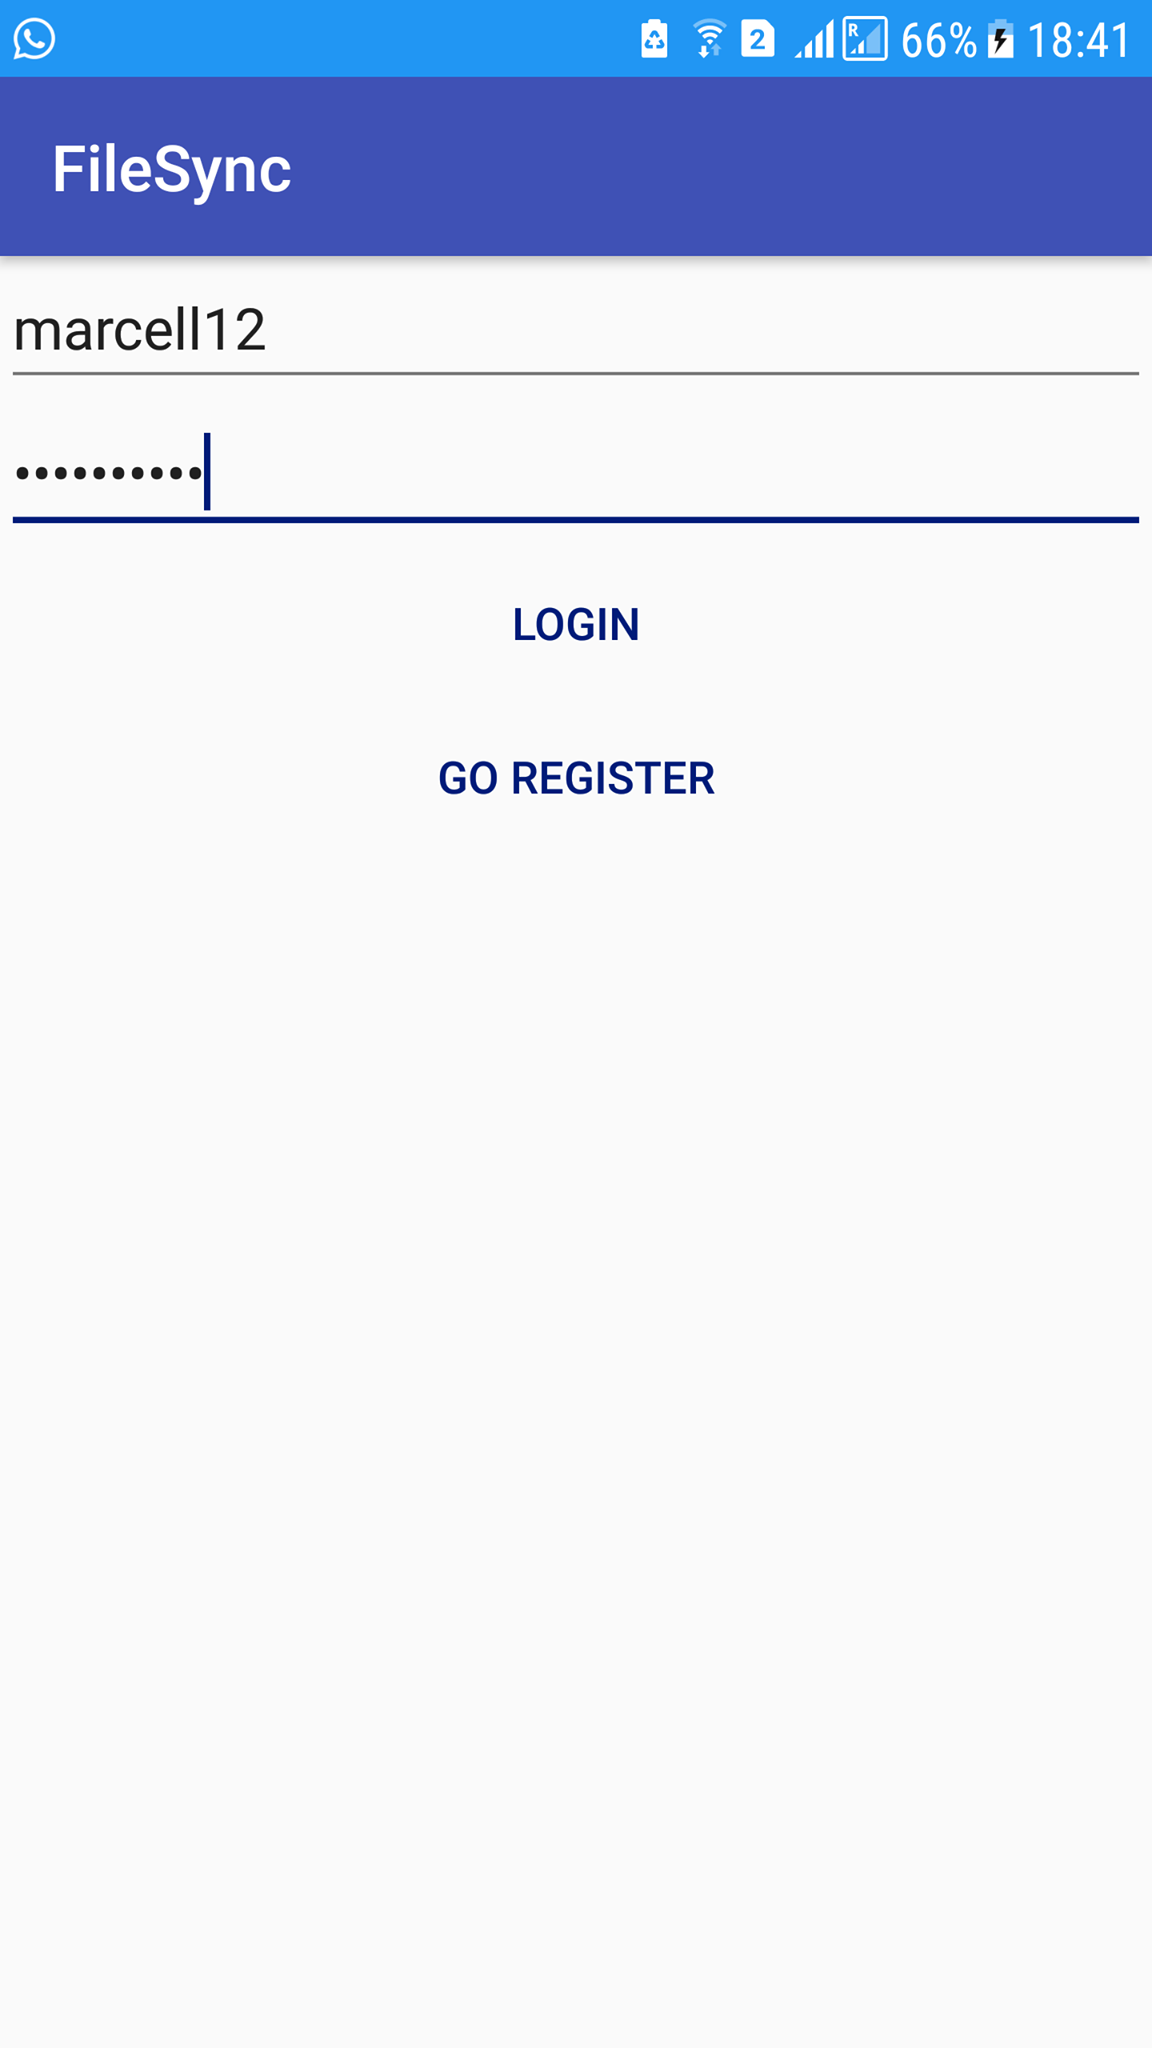
\includegraphics[width=0.3\textwidth]{Group_Project/login.png}
\end{figure}

\begin{figure} [H]
\caption{Android UI to register user account}
\centering
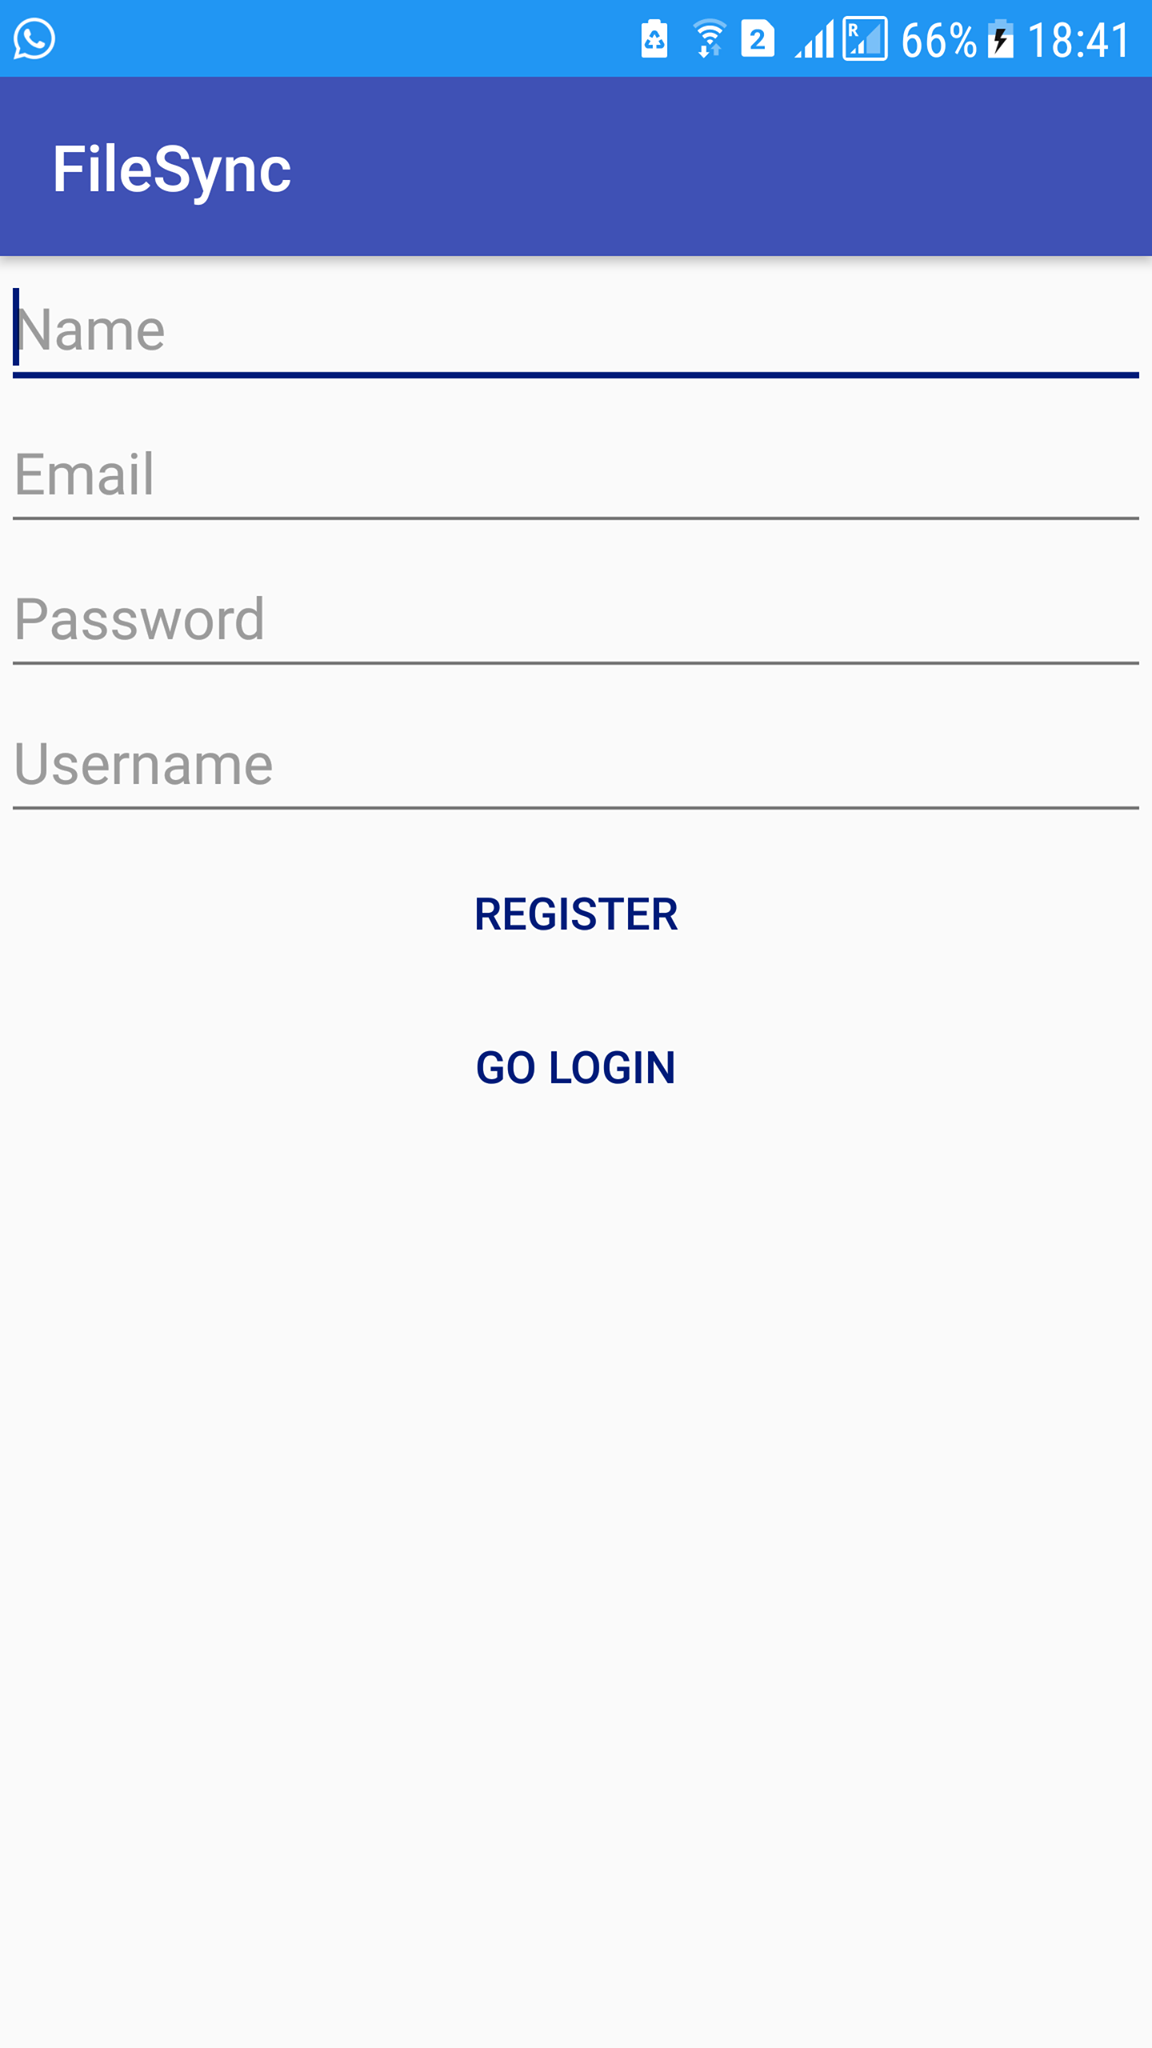
\includegraphics[width=0.3\textwidth]{Group_Project/register.png}
\end{figure}

\begin{figure} [H]
\caption{Android UI to view server files}
\centering
\includegraphics[width=0.3\textwidth]{Group_Project/files.png}
\end{figure}


\begin{figure} [H]
\caption{Android UI to choose file to upload}
\centering
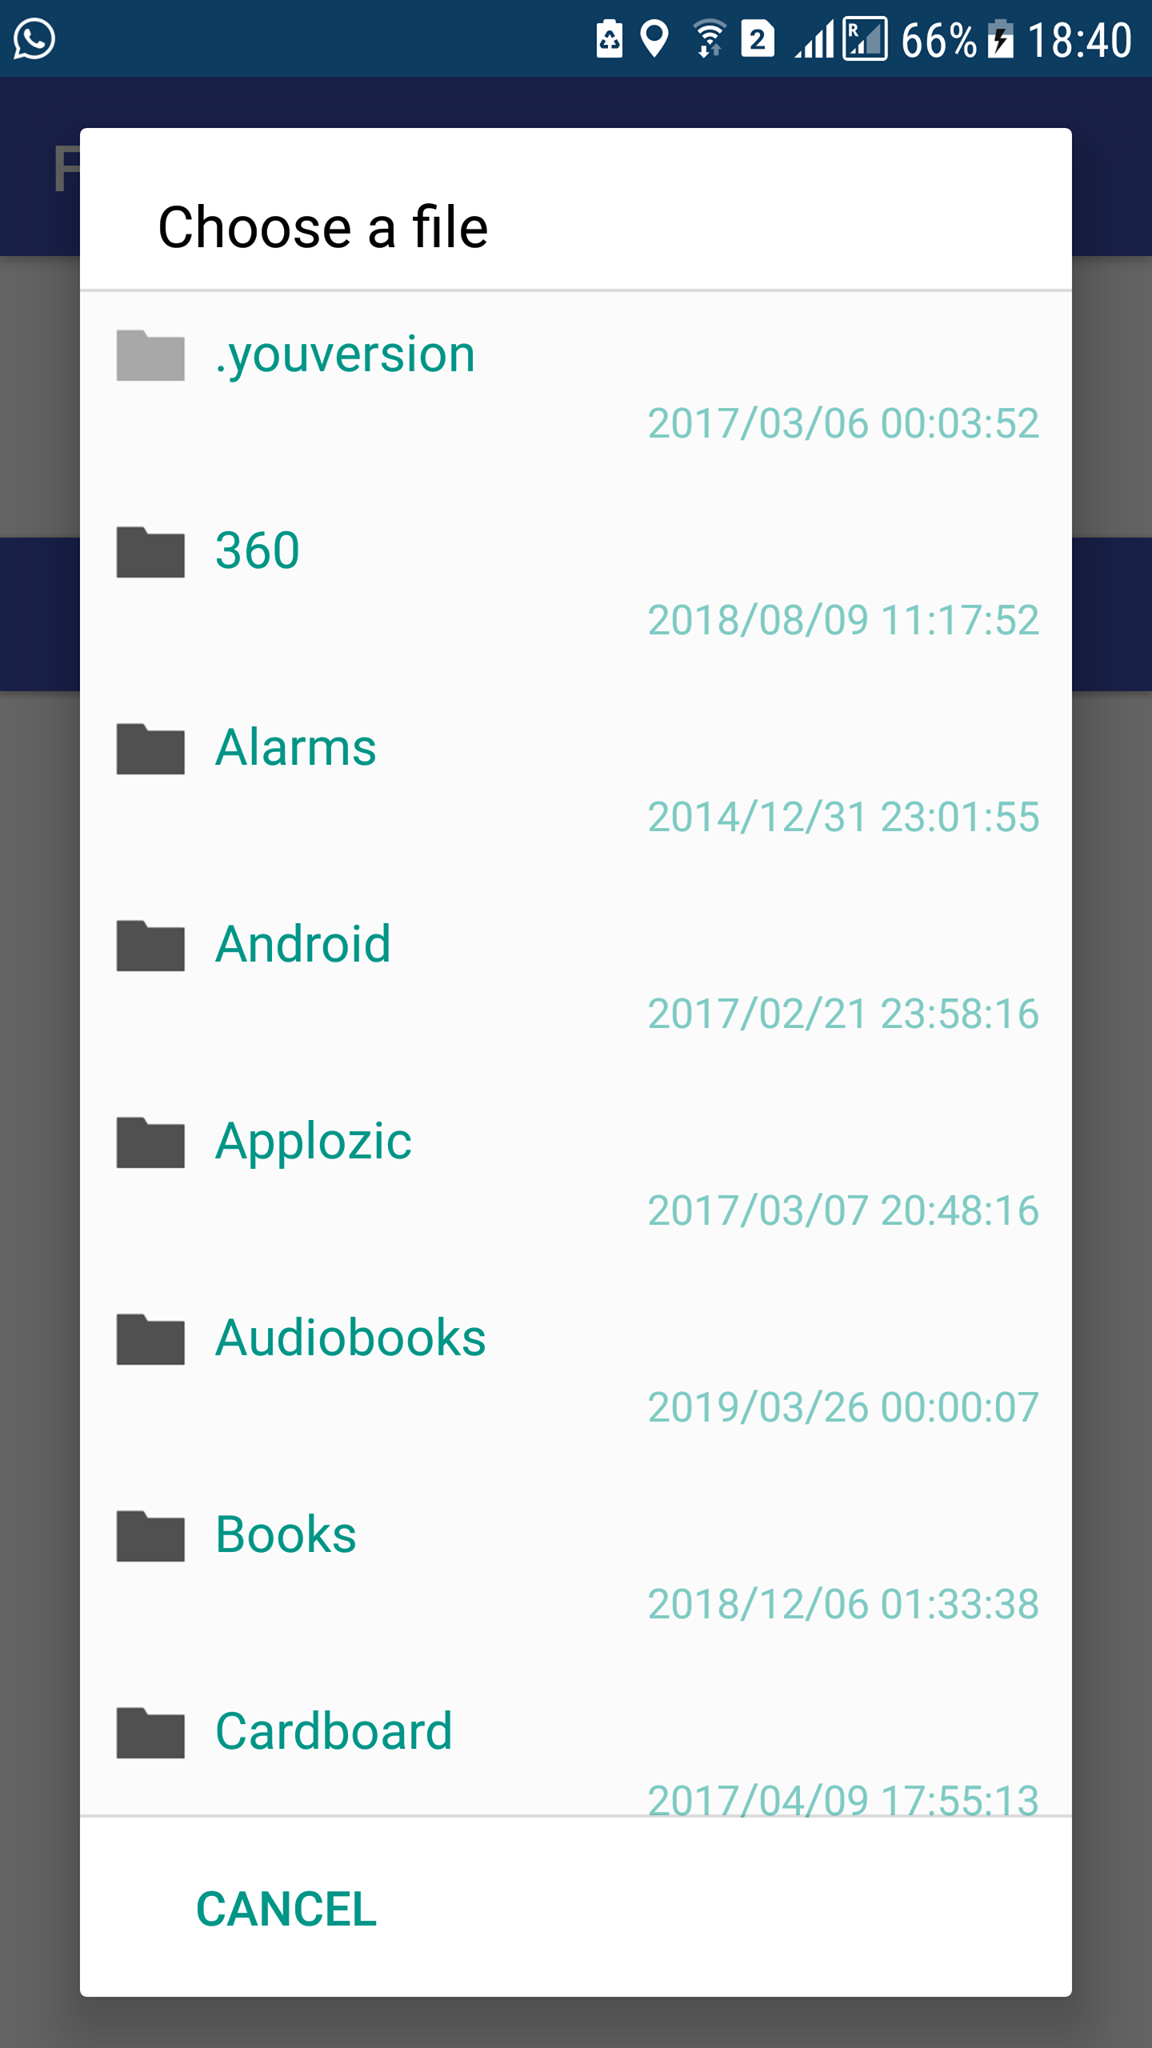
\includegraphics[width=0.3\textwidth]{Group_Project/choose.png}
\end{figure}

\begin{figure} [H]
\caption{Android UI to upload files to server}
\centering
\includegraphics[width=0.3\textwidth]{Group_Project/upload.png}
\end{figure}








\end{document}
